\documentclass[12pt,letterpaper]{article}

\usepackage[T1]{fontenc}
\usepackage[utf8]{inputenc}
\usepackage[spanish,es-nodecimaldot]{babel}
\usepackage{mathptmx}
\usepackage[margin=2.5cm]{geometry}
\usepackage{setspace}
\usepackage{amsmath,amssymb}
\usepackage{booktabs}
\usepackage{graphicx}
\usepackage{caption}
\usepackage[hidelinks]{hyperref}
\usepackage{natbib}
\usepackage{microtype}

\onehalfspacing
\captionsetup{font=small,labelfont=bf}
\setlength{\parskip}{2pt}

\newcommand{\lr}{\ell_{r}}
\newcommand{\lnr}{\ell_{nr}}
\newcommand{\lrt}{\ell_{r,t}}
\newcommand{\lnrt}{\ell_{nr,t}}

\title{\vspace{-1.5cm}\large\textbf{Replicación del resultado principal de\\
Eden y Gaggl (2018), \emph{On the Welfare Implications of Automation}}}
\author{}
\date{\today}

\begin{document}
\maketitle
\vspace{-1cm}

\section{Resumen del artículo original}

\paragraph{Motivación y pregunta de investigación.}
Entre 1950 y 2013 la participación del trabajo en el ingreso de Estados Unidos
cayó de 63,6\% a 57,1\%. La lectura habitual atribuye esa caída a un abaratamiento
del capital frente al trabajo. \citet{eden2018} preguntan algo más fino: ¿cuánto de
esa caída se explica por la \emph{automatización}, entendida como la mecanización
de tareas que antes requerían trabajo, y cuál es el efecto de ese proceso sobre el
bienestar agregado? La pregunta no es obvia porque el capital en tecnologías de la
información y las comunicaciones (TIC) representa una fracción muy pequeña del
ingreso —1,8\% en el modelo calibrado— y un ejercicio de contabilidad del
crecimiento estándar le asignaría, por eso mismo, un papel marginal. El argumento
del artículo es que esa intuición contable subestima el efecto porque ignora la
recomposición de la demanda de trabajo y la acumulación complementaria de capital
no TIC.

\paragraph{Contribución a la literatura.}
El aporte central es separar el capital TIC del capital no TIC (NTIC).
\citet{karabarbounis2014} y \citet{autor2013} trabajan con un agregado único de
capital y \citet{krusell2000} distinguen equipo de estructuras, del cual el capital
TIC es un subconjunto estrecho. La desagregación importa porque la caída de precios
se concentra justo en el capital más sustituible con trabajo: el artículo reproduce
la mitad de la caída del \emph{labor share} con una elasticidad agregada
capital--trabajo de 1,046, mientras que un modelo con capital agregado necesita
valores del orden de 1,25.

\paragraph{Metodología.}
Tres piezas. Una medición: siguiendo \citet{hall1967} y las cuentas detalladas de
activos fijos del BEA, se construyen participaciones de ingreso por tipo de capital
a partir de una condición de no arbitraje entre activos. Una calibración: los cuatro
parámetros de una función CES anidada se estiman por mínimos cuadrados sobre las
condiciones de primer orden de la firma, escritas como relaciones log-lineales entre
participaciones y cantidades relativas. Y una simulación: un modelo de crecimiento
neoclásico con agente representativo, alimentado con las trayectorias observadas del
precio y la depreciación del capital TIC, del que se obtienen la transición
1950--2013 y una medida de bienestar equivalente en consumo.

\paragraph{Resultados principales.}
La participación del capital TIC en el ingreso se multiplicó por siete, de 0,63\% en
1950 a 4,10\% en 2013, mientras que la del capital NTIC no muestra tendencia. Dentro
del trabajo, el ingreso se reasignó de ocupaciones de rutina a ocupaciones de no
rutina. En la simulación, la caída del precio del capital TIC y el alza de su
depreciación generan una caída de 3,46 puntos porcentuales del \emph{labor share},
aproximadamente la mitad de los 6,52 puntos observados, y ganancias de bienestar
del orden de 4\% en consumo permanente. Al mismo tiempo, racionalizar toda la caída
del ingreso de rutina mediante cambios en oferta relativa de factores exige una
elasticidad de sustitución entre trabajo de rutina y no rutina de 7,8, implausiblemente
alta, de donde los autores concluyen que la automatización no puede ser el único
motor de esa recomposición.

\paragraph{Qué aprendemos de economía.}
Tres lecciones. La primera es que la contabilidad del crecimiento subestima de forma
sistemática el aporte de un factor cuando ese factor induce acumulación de otros: en
este modelo el efecto de equilibrio general es $1/(1-\alpha)\approx 1{,}5$ veces el
efecto contable directo, porque más capital TIC eleva el producto marginal del capital
NTIC y atrae inversión complementaria. La segunda es que, para la distribución
funcional del ingreso, importa \emph{cuál} capital se abarata y no solo cuánto: una
caída de precios concentrada en el capital más sustituible con trabajo mueve el
\emph{labor share} mucho más que una caída uniforme. La tercera es una lección sobre
el alcance del agente representativo: el 4\% de ganancia de bienestar es una cota
superior, porque el modelo supone movilidad ocupacional sin costo y no contabiliza
quién gana y quién pierde.

\section{El modelo en detalle}

\subsection{Ambiente económico}

\paragraph{Agentes y preferencias.}
Hay un hogar representativo de horizonte infinito que posee los dos stocks de capital
y una unidad de trabajo, y una firma representativa competitiva. El hogar ordena
sus trayectorias de consumo según
\begin{equation}
\sum_{t=0}^{\infty}\beta^{t}\,\ln(c_{t}), \qquad \beta = 0{,}9737,
\end{equation}
donde $c_t$ es consumo por trabajador. La utilidad logarítmica fija la elasticidad de
sustitución intertemporal en uno, valor consistente con el rango de estimaciones
disponibles y apropiado dado que el ejercicio se enfoca en tendencias de largo plazo.

\paragraph{Tecnología.}
El producto por trabajador se genera con una estructura CES de dos niveles anidada
dentro de una Cobb--Douglas:
\begin{align}
y_{t} &= k_{n,t}^{\alpha}\, x_{t}^{1-\alpha}, \label{eq:y}\\
x_{t} &= \Big[\eta\, \lrt^{\theta} + (1-\eta)\, z_{t}^{\theta}\Big]^{1/\theta}, \label{eq:x}\\
z_{t} &= \Big[\gamma\, k_{c,t}^{\sigma} + (1-\gamma)\, \lnrt^{\sigma}\Big]^{1/\sigma}, \label{eq:z}
\end{align}
con $k_{n}$ capital NTIC, $k_{c}$ capital TIC, $\lr$ trabajo de rutina y $\lnr$ trabajo
de no rutina, todos normalizados por el trabajo agregado.

La estructura no es arbitraria: cada nivel codifica un supuesto económico distinto.
El nivel externo es Cobb--Douglas porque la participación del capital NTIC en el
ingreso no exhibe tendencia en los datos, y una Cobb--Douglas es exactamente la
tecnología que entrega una participación constante. Esto genera una predicción
contrastable fuerte, $s_{n,t}=\alpha$ en todo momento, que usamos más abajo como
prueba de consistencia. El nivel intermedio junta el capital TIC con el trabajo de no
rutina en un compuesto $z$ con elasticidad $1/(1-\sigma)=1{,}427$: son insumos que se
usan conjuntamente, no uno en lugar del otro. El nivel interno enfrenta ese compuesto
contra el trabajo de rutina con elasticidad $1/(1-\theta)=8{,}04$: el trabajo de rutina
es fácilmente reemplazable por el paquete ``computador más trabajador no rutinario'',
y eso es precisamente lo que el modelo entiende por automatización.

\paragraph{Dotaciones.}
El hogar dispone de una unidad de trabajo por período, que reparte entre las dos
ocupaciones, y de stocks iniciales $k_{n,0}$ y $k_{c,0}$. El trabajo agregado $L_t$
crece a tasa constante $g=0{,}0192$, lo que introduce el factor $(1+g)$ en la
acumulación por trabajador. El capital NTIC es el numerario, con precio $p_{n}=1$ y
depreciación constante $\delta_{n}=0{,}0733$.

\paragraph{Fricciones y variación exógena.}
El modelo no tiene fricciones, y la ausencia es deliberada. El trabajo es homogéneo y
se reasigna entre ocupaciones sin costo, no hay costos de ajuste del capital, ni
búsqueda, ni rigideces nominales, ni heterogeneidad de agentes. Los autores eligen
este ambiente por dos razones: porque las especificaciones con trabajo diferenciado
producen $\theta>1$, inconsistente con el marco CES, y porque un ambiente sin
fricciones entrega naturalmente una \emph{cota superior} de las ganancias de
bienestar, que es el objeto de interés. Las únicas rigideces son tecnológicas: las
elasticidades de sustitución finitas de \eqref{eq:x} y \eqref{eq:z}.

La única variación exógena son dos series: el precio relativo del capital TIC
$p_{c,t}$, interpretable como la tasa a la que el producto se transforma en capital
TIC, y su tasa de depreciación $\delta_{c,t}$. Juntas capturan el precio efectivo del
capital TIC desde el punto de vista de un inversionista.

\subsection{Problemas de optimización}

\paragraph{Problema del hogar.}
El hogar elige $\{c_t, k_{n,t+1}, k_{c,t+1}, \lrt, \lnrt\}$ para maximizar (1)
sujeto a \eqref{eq:y}--\eqref{eq:z}, a $\lrt+\lnrt=1$ y a la restricción
presupuestaria
\begin{equation}
c_{t} + (1+g)\sum_{i=n,c} p_{i,t}\,k_{i,t+1}
\;=\; y_{t} + \sum_{i=n,c} p_{i,t}\,(1-\delta_{i,t})\,k_{i,t}.
\label{eq:bc}
\end{equation}

\paragraph{Condiciones de primer orden.}
Con $\lambda_t$ el multiplicador de \eqref{eq:bc} y $\mu_t$ el de la restricción de
trabajo, las condiciones son
\begin{align}
\frac{1}{c_{t}} &= \lambda_{t}, \label{eq:foc_c}\\
\frac{\partial y_{t}}{\partial \lrt} &= \frac{\partial y_{t}}{\partial \lnrt}
\;=\; \frac{\mu_{t}}{\lambda_{t}} \;\equiv\; w_{t}, \label{eq:foc_l}\\
(1+g)\,p_{i,t}\,\lambda_{t} &= \beta\,\lambda_{t+1}
\left[\frac{\partial y_{t+1}}{\partial k_{i,t+1}} + p_{i,t+1}(1-\delta_{i,t+1})\right],
\quad i=n,c. \label{eq:euler}
\end{align}
Derivando \eqref{eq:y}--\eqref{eq:z}, los productos marginales son
\begin{align}
\frac{\partial y}{\partial k_{n}} = \alpha\,\frac{y}{k_{n}},
\qquad
\frac{\partial y}{\partial \lr} &= (1-\alpha)\frac{y}{x}\;\eta\Big(\frac{x}{\lr}\Big)^{1-\theta},\\
\frac{\partial y}{\partial k_{c}} &= (1-\alpha)\frac{y}{x}\,(1-\eta)\Big(\frac{x}{z}\Big)^{1-\theta}\gamma\Big(\frac{z}{k_{c}}\Big)^{1-\sigma},\\
\frac{\partial y}{\partial \lnr} &= (1-\alpha)\frac{y}{x}\,(1-\eta)\Big(\frac{x}{z}\Big)^{1-\theta}(1-\gamma)\Big(\frac{z}{\lnr}\Big)^{1-\sigma}.
\end{align}

\paragraph{Interpretación económica.}
La ecuación \eqref{eq:foc_l} es el corazón del mecanismo. Como el trabajo es homogéneo
y móvil, el hogar reparte su unidad de trabajo hasta igualar productos marginales, de
modo que un mismo salario $w_t$ rige en ambas ocupaciones y toda la diferencia entre
las participaciones de ingreso de rutina y no rutina refleja diferencias en
\emph{cantidades} de trabajo, no en precios. Cuando $p_{c,t}$ cae, el hogar acumula
capital TIC; ese capital entra en $z$, eleva el producto marginal del trabajo de no
rutina —su complemento en \eqref{eq:z}— y, dado que $z$ y $\lr$ son muy sustituibles
en \eqref{eq:x}, deprime el del trabajo de rutina. La igualación de \eqref{eq:foc_l}
se restablece entonces trasladando trabajadores de rutina hacia no rutina. Eso es la
automatización en este modelo: no una destrucción de empleo, sino una recomposición
ocupacional inducida por precios de capital.

La ecuación \eqref{eq:euler} es la de Euler estándar, escrita por tipo de capital.
Su lado izquierdo es el costo en utilidad de renunciar hoy a $p_{i,t}$ unidades de
consumo; el derecho, el beneficio descontado de la renta más el valor de reventa neto
de depreciación. Que se cumpla para $i=n$ y $i=c$ simultáneamente es lo que fuerza la
no arbitraje entre ambos activos, y es también la relación que \citet{eden2018} usan
en la parte empírica para recuperar las participaciones de ingreso por tipo de capital.

\subsection{Equilibrio}

\paragraph{Definición.}
Dados los stocks iniciales $(k_{n,0},k_{c,0})$ y las secuencias exógenas
$\{p_{c,t},\delta_{c,t}\}_{t\ge 0}$, un \emph{equilibrio competitivo con previsión
perfecta} es un conjunto de secuencias de cantidades
$\{c_{t},k_{n,t+1},k_{c,t+1},\lrt,\lnrt\}$ y de precios $\{w_{t},R_{n,t},R_{c,t}\}$
tales que: (i) las cantidades resuelven el problema del hogar tomando los precios
como dados; (ii) la firma maximiza beneficios, lo que con retornos constantes a
escala implica que los precios de los factores igualan sus productos marginales y
que los beneficios son nulos; (iii) los mercados se vacían.

\paragraph{Vaciado de mercados.}
El mercado de trabajo exige $\lrt+\lnrt=1$; los de alquiler de capital, que la
demanda de cada tipo iguale el stock disponible $k_{i,t}$; y el de bienes,
\begin{equation}
c_{t} + (1+g)\big(k_{n,t+1} + p_{c,t}k_{c,t+1}\big)
= y_{t} + (1-\delta_{n})k_{n,t} + p_{c,t}(1-\delta_{c,t})k_{c,t}.
\label{eq:rc}
\end{equation}
Por la ley de Walras, \eqref{eq:rc} es redundante dadas las demás condiciones y la
restricción del hogar.

\paragraph{Caracterización.}
Como no hay distorsiones, se cumplen los teoremas del bienestar y la asignación
coincide con la del planificador. Sustituyendo \eqref{eq:foc_c} en \eqref{eq:euler}
y usando \eqref{eq:rc} para eliminar $c_t$, el equilibrio queda caracterizado por un
sistema de ecuaciones en diferencias de segundo orden en $(k_{n,t},k_{c,t})$, con
condición inicial dada y condición terminal de transversalidad.

En estado estacionario las variables por trabajador son constantes y \eqref{eq:euler}
colapsa a la igualdad entre producto marginal y costo de uso. Siguiendo la convención
del artículo, en la cual la ecuación de Euler de largo plazo se escribe
$\beta(1+r)=1$, el retorno requerido es $r=1/\beta-1=2{,}70\%$ y
\begin{equation}
\frac{\partial y}{\partial k_{i}} \;=\; p_{i}\left(\frac{1}{\beta}-1+\delta_{i}\right),
\qquad i=n,c.
\label{eq:ss}
\end{equation}
Junto con \eqref{eq:foc_l} y $\lr+\lnr=1$, \eqref{eq:ss} forma un sistema de tres
ecuaciones en tres incógnitas $(k_{n},k_{c},\lr)$. Dos propiedades del estado
estacionario se usan más adelante como controles: de \eqref{eq:ss} con $i=n$ se sigue
$s_{n}=\alpha$ exactamente y en todo momento, y de \eqref{eq:y} se sigue
$\ln k_{n} = \text{cte} + \ln x$, es decir, el capital NTIC sigue uno a uno al
compuesto $x$. Esta segunda propiedad es la que genera la amplificación de equilibrio
general: el efecto total del capital TIC sobre el producto es $1/(1-\alpha)\approx1{,}54$
veces su efecto contable directo.

\section{Estrategia de solución}

\paragraph{Método numérico.}
El modelo es determinístico y con previsión perfecta, de modo que no hay valor
esperado que aproximar ni espacio de estados que discretizar: no se requiere
programación dinámica. Se resuelve por el método de tiempo apilado
(\emph{stacked-time}) de \citet{laffargue1990} y \citet{boucekkine1995}, el mismo que
usa Dynare en su rutina de previsión perfecta: se escriben todas las ecuaciones de
Euler del horizonte como un único sistema no lineal y se resuelve con Newton.

\paragraph{Discretización.}
La única discretización es temporal. Se trunca el horizonte en $T=160$ años y se impone
como condición terminal $k_{i,T+1}=k_{i}^{ee,\text{final}}$, que es la contraparte
numérica de la transversalidad. Las series exógenas se mantienen constantes después de
2013, de manera que la economía converge al estado estacionario final mucho antes de
$T$; se verificó que duplicar $T$ deja los resultados inalterados en todas las cifras
reportadas. El consumo no es una incógnita del sistema: se recupera período a período
de \eqref{eq:rc}, lo que reduce el tamaño del problema a $2(T-1)=318$ incógnitas.

\paragraph{Algoritmo.}
\begin{enumerate}\setlength{\itemsep}{0pt}
\item Calibrar por bisección el nivel de productividad $A$ que fija la escala, de modo
que el producto del estado estacionario inicial satisfaga $\ln y = 10{,}20$.
\item Resolver los tres estados estacionarios relevantes —inicial, final de la
simulación base y final del contrafactual— con un Newton amortiguado sobre
\eqref{eq:foc_l} y \eqref{eq:ss}, en las variables $(\ln k_{n}, \ln k_{c},
\operatorname{logit}\lr)$ para imponer los dominios.
\item Construir la semilla de la transición por interpolación log-lineal entre los
estados estacionarios inicial y final.
\item Dado un vector candidato de capital, resolver en cada período la asignación
estática del trabajo \eqref{eq:foc_l} mediante un Newton escalar sobre
$\operatorname{logit}\lrt$, vectorizado sobre los $T+1$ períodos.
\item Obtener $\{c_t\}$ de \eqref{eq:rc} y evaluar los $2(T-1)$ residuos de Euler.
\item Construir el jacobiano por diferencias centradas. El residuo del período $t$
depende únicamente del capital en $t$, $t+1$ y $t+2$, de modo que el jacobiano es de
banda angosta; se explota con coloreo a la \citet{curtis1974}, perturbando
simultáneamente variables separadas por trece posiciones, cuyos soportes de filas son
disjuntos. El jacobiano completo cuesta 26 evaluaciones del residuo en lugar de 636.
\item Dar el paso de Newton con búsqueda de línea por bisección sobre la norma
euclidiana del residuo, y repetir desde el paso 4.
\end{enumerate}

\paragraph{Criterios de convergencia.}
El criterio principal es $\max_{t,i}|R_{i,t}|<10^{-10}$ sobre los residuos de Euler
expresados en forma relativa, es decir, como errores de Euler adimensionales
interpretables como el porcentaje de consumo que el hogar desperdicia al seguir la
solución numérica en vez de la exacta. Los criterios auxiliares son $10^{-13}$ para la
asignación intratemporal del trabajo y $10^{-12}$ para la bisección de $A$. La
transición base converge en 5 iteraciones de Newton con residuo final
$3{,}1\times10^{-13}$.

\paragraph{Validación.}
La solución se somete a cuatro pruebas independientes, reportadas por el código en
\texttt{out/diagnostics.txt}.
\begin{enumerate}\setlength{\itemsep}{0pt}
\item \emph{Consistencia interna}: se simula un contrafactual en el que $p_{c,t}$ y
$\delta_{c,t}$ se mantienen constantes. El solver de transición debe devolver
exactamente el estado estacionario inicial en todos los períodos. Desvío máximo
obtenido: $1{,}7\times10^{-10}$.
\item \emph{Agotamiento del producto}: con retornos constantes a escala las cuatro
participaciones deben sumar uno en cada período. Desvío máximo:
$4{,}4\times10^{-16}$.
\item \emph{Restricción teórica}: la Cobb--Douglas externa implica $s_{n,t}=\alpha$
para todo $t$. El código lo verifica y obtiene $35{,}05\%$ constante.
\item \emph{Coherencia entre solvers}: el último período de la transición debe
coincidir con el estado estacionario final calculado de forma independiente. Diferencia
en $\ln k_{n}$ y $\ln k_{c}$: $1{,}1\times10^{-6}$.
\end{enumerate}

\section{Resultados de la replicación}

\subsection{Resultado principal replicado}

El resultado replicado es la Tabla 4 del artículo, que compara el estado estacionario
inicial (precio y depreciación del capital TIC de 1950) con el final de la simulación
base (valores de 2013) y con el del contrafactual en que el precio del capital TIC se
mantiene constante. El Cuadro \ref{tab:t4} reproduce sus cuatro paneles junto a las
cifras originales.

\begin{table}[t]\centering
\caption{Replicación de la Tabla 4 de \citet{eden2018}}
\label{tab:t4}
\small
\begin{tabular}{lrrrrrr}
\toprule
& \multicolumn{3}{c}{\textbf{Replicación}} & \multicolumn{3}{c}{\textbf{Original}}\\
\cmidrule(lr){2-4}\cmidrule(lr){5-7}
& EE inicial & EE final & Contraf. & EE inicial & EE final & Contraf.\\
\midrule
\multicolumn{7}{l}{\emph{A. Producto y consumo}}\\
$\ln y$ & 10,20 & 10,34 & 10,19 & 10,20 & 10,34 & 10,19\\
$\ln c$ & \phantom{0}9,78 & \phantom{0}9,87 & \phantom{0}9,77 & \phantom{0}9,79 & \phantom{0}9,87 & \phantom{0}9,78\\
\addlinespace
\multicolumn{7}{l}{\emph{B. Capital}}\\
$\ln k_{c}$ & \phantom{0}7,45 & 10,22 & \phantom{0}6,85 & \phantom{0}7,46 & 10,22 & \phantom{0}6,86\\
$\ln k_{n}$ & 11,45 & 11,59 & 11,44 & 11,45 & 11,59 & 11,44\\
\addlinespace
\multicolumn{7}{l}{\emph{C. Participación del trabajo (\%)}}\\
Agregada & 63,15 & 59,70 & 63,51 & 63,14 & 59,68 & 63,51\\
Rutina & 35,60 & 19,96 & 37,92 & 35,58 & 19,98 & 37,93\\
No rutina & 27,55 & 39,74 & 25,59 & 27,55 & 39,71 & 25,58\\
\addlinespace
\multicolumn{7}{l}{\emph{D. Participación del capital TIC (\%)}}\\
TIC & \phantom{0}1,80 & \phantom{0}5,25 & \phantom{0}1,44 & \phantom{0}1,81 & \phantom{0}5,27 & \phantom{0}1,44\\
\midrule
\multicolumn{7}{l}{\emph{Cambios entre estados estacionarios}}\\
$\Delta$ \emph{labor share} (pp) & \multicolumn{3}{c}{$-3{,}45$} & \multicolumn{3}{c}{$-3{,}46$}\\
$\Delta$ participación TIC (pp) & \multicolumn{3}{c}{$+3{,}45$} & \multicolumn{3}{c}{$+3{,}46$}\\
$100\times\Delta\ln y$ & \multicolumn{3}{c}{$13{,}80$} & \multicolumn{3}{c}{$13{,}77$}\\
$100\times\Delta\ln c$ & \multicolumn{3}{c}{$8{,}58$} & \multicolumn{3}{c}{$8{,}47$}\\
$100\times\Delta\ln k_{c}$ & \multicolumn{3}{c}{$277{,}28$} & \multicolumn{3}{c}{$276{,}66$}\\
$100\times\Delta\ln k_{n}$ & \multicolumn{3}{c}{$13{,}80$} & \multicolumn{3}{c}{$13{,}65$}\\
\bottomrule
\end{tabular}
\end{table}

El mensaje sustantivo se replica sin ambigüedad. La caída del precio del capital TIC y
el alza de su depreciación reducen la participación del trabajo en $3{,}45$ puntos
porcentuales, frente a los $3{,}46$ del artículo, es decir, aproximadamente la mitad de
los $6{,}52$ puntos observados en los datos entre 1950 y 2013. La recomposición interna
del trabajo también se reproduce: la participación de las ocupaciones de rutina cae
$15{,}6$ puntos y la de no rutina sube $12{,}2$, de manera que cerca de cuatro quintas
partes de lo que pierde el trabajo de rutina lo recibe el trabajo de no rutina y solo
el resto se traslada al capital TIC.

La Figura \ref{fig:f7} presenta las trayectorias de transición correspondientes a la
Figura 7 del artículo.

\begin{figure}[t]\centering
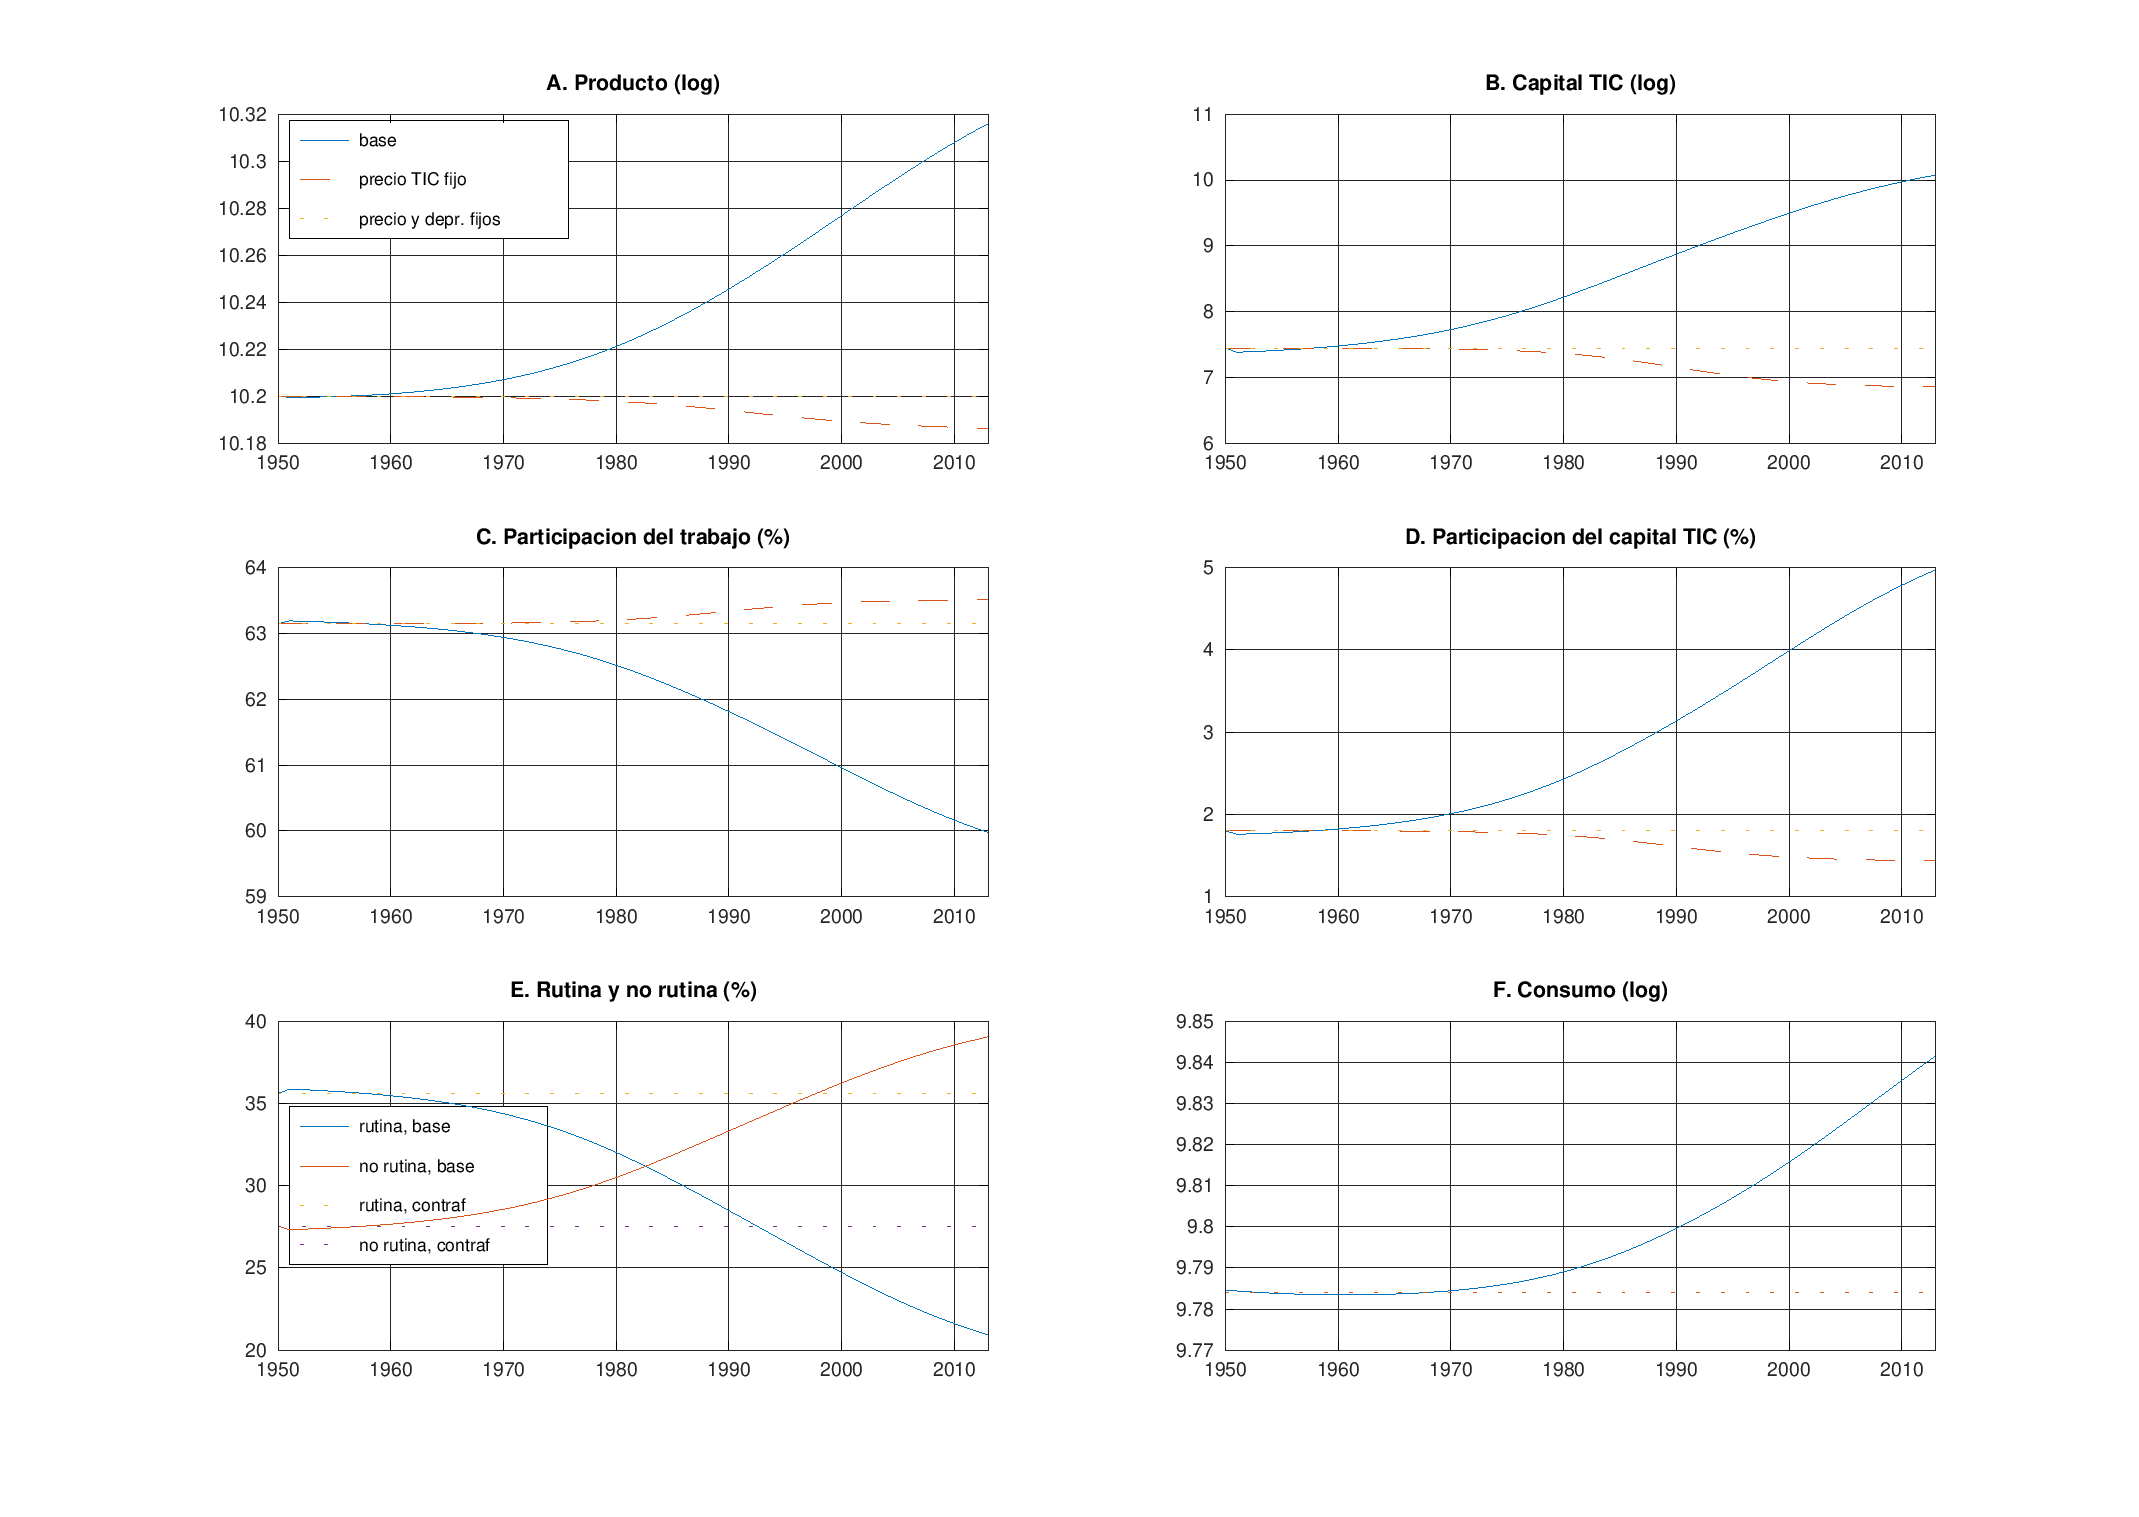
\includegraphics[width=0.96\textwidth]{fig7.png}
\caption{Simulación base y contrafactuales, 1950--2013. Línea continua: simulación
base. Líneas punteadas: contrafactual con precio del capital TIC constante y
contrafactual con precio y depreciación constantes.}
\label{fig:f7}
\end{figure}

\subsection{Comparación con el original}

\paragraph{Diferencias encontradas.}
En los cuatro paneles del Cuadro \ref{tab:t4} ninguna celda se aparta del original en
más de $0{,}03$ puntos porcentuales o $0{,}01$ en logaritmos. Las diferencias más
visibles están en las tasas de cambio: $8{,}58\%$ contra $8{,}47\%$ en consumo y
$277{,}3\%$ contra $276{,}7\%$ en capital TIC. La discrepancia material está en la
medida de bienestar: $\lambda$ evaluada en 1980 da $4{,}75\%$ frente al ``aproximadamente
4\%'' que reporta el artículo.

\paragraph{Posibles explicaciones.}
Las diferencias del Cuadro \ref{tab:t4} son de redondeo y no de método. Los parámetros
publicados vienen con tres o cuatro dígitos: $\gamma$ y $\eta$ se recuperaron de las
constantes de regresión de la Tabla 2 ($-5{,}201$ y $0{,}138$) en vez de los valores
redondeados $0{,}005$ y $0{,}535$ que aparecen impresos, precisamente porque usar estos
últimos desplazaba las participaciones en alrededor de tres décimas de punto. El
residuo que queda es consistente con la precisión de $\alpha$, $\beta$, $\delta_{n}$ y
$g$.

La brecha en $\lambda$ tiene otro origen y conviene ser explícito al respecto. El valor
de $\lambda$ depende de la \emph{trayectoria anual completa} de $p_{c,t}$ y
$\delta_{c,t}$, no solo de sus extremos, porque el descuento hace que importe cuándo
ocurre la caída de precios. Las cuentas detalladas de activos fijos del BEA no
estuvieron disponibles para este ejercicio, de modo que ambas series se aproximaron con
trayectorias logísticas ancladas en los rangos que reporta la Tabla 3 del artículo,
$p_{c}\in[0{,}254,\,1{,}727]$ y $\delta_{c}\in[0{,}137,\,0{,}206]$, y en el calendario
que describe su Sección 5: precio plano a comienzos de los cincuenta, caída rápida
desde comienzos de los sesenta, aplanamiento a mediados de los dos mil; depreciación
plana al inicio y al final, con alza concentrada entre 1980 y 2000. Una caída de
precios que en la aproximación ocurre algo más temprano que en los datos adelanta las
ganancias de consumo y eleva $\lambda$ evaluada en 1980. Nótese que este problema no
afecta al Cuadro \ref{tab:t4}, que solo usa los valores inicial y final y por eso
coincide con el original hasta la segunda cifra decimal.

El perfil de $\lambda$ por cohorte sí reproduce el patrón del artículo: la ganancia
sube de $2{,}1\%$ para quienes optimizan en 1950 a $8{,}3\%$ para quienes lo hacen en
2013. La razón económica es la que señalan \citet{eden2018}: las generaciones tempranas
pagan el costo de la acumulación de capital en consumo sacrificado y además descuentan
unas ganancias que solo se materializan décadas después, mientras que las tardías
heredan el stock ya acumulado.

\paragraph{Alcance.}
Dos resultados del artículo quedan fuera de esta replicación por falta de acceso a los
microdatos. Las columnas de rutina y no rutina de su Tabla 1 requieren extractos del
\emph{Current Population Survey} vía IPUMS, y la calibración de su Tabla 2 requiere
además las cuentas detalladas del BEA. Aquí esos parámetros se tomaron como dados y el
ejercicio se concentró en el bloque estructural, que es el que la simulación produce de
forma endógena.

\small
\begin{thebibliography}{9}
\setlength{\itemsep}{0pt}\setlength{\parskip}{0pt}
\bibitem[Autor y Dorn(2013)]{autor2013} Autor, D. y D. Dorn (2013). ``The Growth of Low-Skill Service Jobs and the Polarization of the US Labor Market''. \emph{American Economic Review} 103(5), 1553--1597.
\bibitem[Boucekkine(1995)]{boucekkine1995} Boucekkine, R. (1995). ``An Alternative Methodology for Solving Nonlinear Forward-Looking Models''. \emph{Journal of Economic Dynamics and Control} 19(4), 711--734.
\bibitem[Curtis et al.(1974)]{curtis1974} Curtis, A., M. Powell y J. Reid (1974). ``On the Estimation of Sparse Jacobian Matrices''. \emph{IMA Journal of Applied Mathematics} 13(1), 117--119.
\bibitem[Eden y Gaggl(2018)]{eden2018} Eden, M. y P. Gaggl (2018). ``On the Welfare Implications of Automation''. \emph{Review of Economic Dynamics} 29, 15--43.
\bibitem[Hall y Jorgenson(1967)]{hall1967} Hall, R. y D. Jorgenson (1967). ``Tax Policy and Investment Behavior''. \emph{American Economic Review} 57(3), 391--414.
\bibitem[Karabarbounis y Neiman(2014)]{karabarbounis2014} Karabarbounis, L. y B. Neiman (2014). ``The Global Decline of the Labor Share''. \emph{Quarterly Journal of Economics} 129(1), 61--103.
\bibitem[Krusell et al.(2000)]{krusell2000} Krusell, P., L. Ohanian, J.-V. Ríos-Rull y G. Violante (2000). ``Capital-Skill Complementarity and Inequality''. \emph{Econometrica} 68(5), 1029--1053.
\bibitem[Laffargue(1990)]{laffargue1990} Laffargue, J.-P. (1990). ``Résolution d'un modèle macroéconomique avec anticipations rationnelles''. \emph{Annales d'Économie et de Statistique} 17, 97--119.
\end{thebibliography}

\end{document}
